Das Linsensystem in Abbildung~\ref{10000057:fig} sieht von aussen wir
ein gewöhnliche Glasscheibe aus: beide Seiten sind flach.
Die gekrümmten Flächen der Linsen haben die gleiche Krümmung.
Die verwendeen Gläser haben jedoch verschiedenen Brechungsindex, so dass
sie trotzdem wie eine Sammellinse wirken. 
Verwenden Sie die paraxiale Näherung (Matrixoptik), um die Brennweite
des Systems zu berechnen.

\begin{figure}[h]
\centering
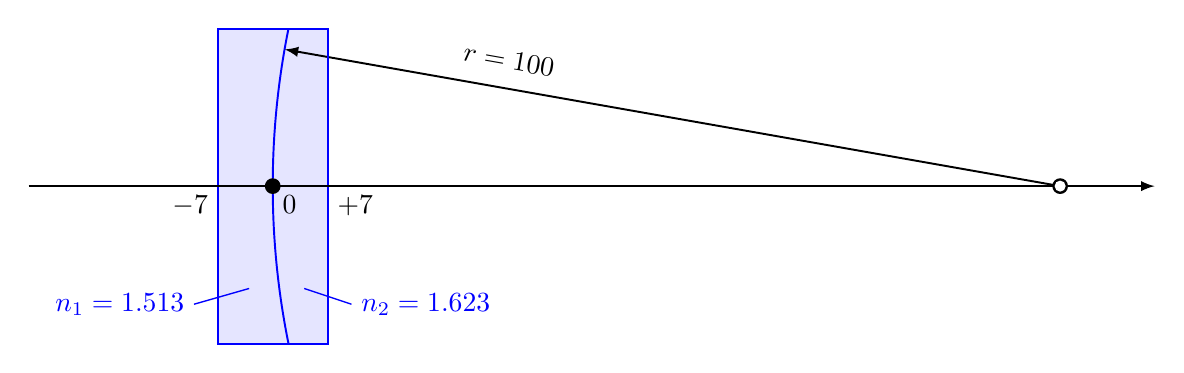
\begin{tikzpicture}[>=latex]
\def\d{0.7}
\fill[color=blue!10] (-\d,-2) rectangle (\d,2);
\begin{scope}
\clip (-\d,-2) rectangle (\d,2);
\draw[line width=0.7pt,color=blue] (10,0) circle[radius=10];
\end{scope}
\begin{scope}
\clip (0,-2) rectangle (11,2);
\draw[line width=0.7pt,->] (10,0) -- ({10*(1-cos(10))},{10*sin(10)});
\end{scope}
\node at (3,1.6) [rotate=-10] {$r = 100$};
\draw[color=blue,line width=0.7pt] (-\d,-2)--(\d,-2)--(\d,2)--(-\d,2)--cycle;
\draw[->,line width=0.7pt] (-3.1,0)--(11.2,0);
\node at (0.7,0) [below right] {$+7$};
\node at (-0.7,0) [below left] {$-7$};
\draw[line width=0.7pt] (-0.7,0.08)--(-0.7,0.08);
\draw[line width=0.7pt] (0.7,0.08)--(0.7,0.08);
\node at (0, 0) [below right] {$0$};
\fill (0,0) circle[radius=0.1];
\node[color=blue] at (-1,-1.5) [left] {$n_1 = 1.513$};
\node[color=blue] at (1,-1.5) [right] {$n_2 = 1.623$};
\draw[line width=0.5pt,color=blue] (-0.3,-1.3)--(-1,-1.5);
\draw[line width=0.5pt,color=blue] (0.4,-1.3)--(1,-1.5);
%\fill[color=red] (-3,1) circle[radius=0.1];
\fill (10,0) circle[radius=0.1];
\fill[color=white] (10,0) circle[radius=0.07];
\end{tikzpicture}
\caption{Linsensystem für Aufgabe~\ref{10000057}
\label{10000057:fig}}
\end{figure}

\begin{loesung}
Zunächst müssen wir die Transfermatrix des Gesamtsystems aus den Matrizen
der einzelnen gekrümmten Flächen berechnen.
Wegen des unendlichen Krümmungsradius sind die Transfermatrizen für 
die Aussenflächen des Systems
\[
B_1=B(1,n_1,\infty) = \begin{pmatrix} 1&0\\0&n_1^{-1}\end{pmatrix}
\qquad\text{und}\qquad
B_3=B(n_2,1,\infty) = \begin{pmatrix} 1&0\\0&n_2\end{pmatrix}.
\]
Die Brechung an der gekrümmten Fläche ist
\[
B_2 = B(n_1,n_2,r)
=
\begin{pmatrix}
1&0\\
\frac1r(\nu -1) & \nu
\end{pmatrix}
\qquad
\text{mit}\quad
\nu = \frac{n_1}{n_2}.
\]


Um die Brennweite zu finden, berechnen wir den Punkt $(f,0)$, durch den
ein von $(-1,1)$ ausgehender horizontaler Strahl hindurchgeht.
In solcher wird durch den Vektor
\[
\begin{pmatrix}1\\0\end{pmatrix}
\]
beschrieben.
Dieser Strahl entwickelt sich erst mit der Matrix $T_{l_1}$ über die Distanz
$l_1 = 23$ bis er auf der linken planen Fläche auftrifft.
Dort wird er mit der Matrix $B_1$ gebrochen und bewegt sich dann
weiter mit $T_{7}$ bis zur gekrümmten Fläche.
Es folgt $B_2$, $T_7$, $B_3$ und schliesslich $T_{f-z}$.
Am Ende all dieser Transformationen kreuzt der Strahl die $x$-Achse, die erste
Komponente des Vektors verschwindet daher.
Es muss also $f$ so gefunden werden, dass
\[
T_{f-7}
B_3
T_{7}
B_2
T_{7}
B_1
T_{23}
\begin{pmatrix}1\\0\end{pmatrix}
=
\begin{pmatrix} 0 \\ ? \end{pmatrix}.
\]
Setzen wir alle Definition ein, erhalten wir
\begin{align*}
\begin{pmatrix}0\\?\end{pmatrix}
&=
\begin{pmatrix}1&f-7\\0&1\end{pmatrix}
\begin{pmatrix}1&0\\0&n_2\end{pmatrix}
\begin{pmatrix}1&7\\0&1\end{pmatrix}
\begin{pmatrix}1&0\\\frac1r(\nu-1)&\nu\end{pmatrix}
\begin{pmatrix}1&7\\0&1\end{pmatrix}
\begin{pmatrix}1&0\\0&1/n_1\end{pmatrix}
\begin{pmatrix}1&23\\0&1\end{pmatrix}
\begin{pmatrix}1\\0\end{pmatrix}
\\
&=
\begin{pmatrix}1&f-7\\0&1\end{pmatrix}
\begin{pmatrix}1&0\\0&n_2\end{pmatrix}
\begin{pmatrix}1&7\\0&1\end{pmatrix}
\begin{pmatrix}1&0\\\frac1r(\nu-1)&\nu\end{pmatrix}
\begin{pmatrix}1\\0\end{pmatrix}
\\
&=
\begin{pmatrix}1&f-7\\0&1\end{pmatrix}
\begin{pmatrix}1&0\\0&n_2\end{pmatrix}
\begin{pmatrix}1&7\\0&1\end{pmatrix}
\begin{pmatrix}1\\\frac1r(\nu-1)\end{pmatrix}
\\
&=
\begin{pmatrix}1&f-7\\0&1\end{pmatrix}
\begin{pmatrix}1&0\\0&n_2\end{pmatrix}
\begin{pmatrix}1+\frac7r(\nu-1)\\\frac1r(\nu-1)\end{pmatrix}
\\
&=
\begin{pmatrix}1&f-7\\0&1\end{pmatrix}
\begin{pmatrix}1+\frac7r(\nu-1)\\n_2\frac1r(\nu-1)\end{pmatrix}
\\
&=
\begin{pmatrix}
1+\frac7r(\nu-1)
+
(f-7)(n_2\frac1r(\nu-1))
\\
n_2\frac1r(\nu-1)
\end{pmatrix}.
\end{align*}
Die erste Komponente dieses Vektors muss verschwinden, es gilt daher
\begin{align*}
1+\frac7r(\nu-1)
+
(f-7)(n_2\frac1r(\nu-1))
&=
0
\\
f-7
&=
-\frac{1+\frac7r(\nu-1)}{ n_2\frac1r(\nu-1) }
\\
f
&=
7
+\frac{1+\frac7r(\nu-1)}{ n_2\frac1r(\nu-1) }
=
7
+\frac{r+7(\nu-1)}{ n_2(\nu-1) }
\\
&=
7
+\frac{r+7(\nu-1)}{ n_1 -n_2 }
\end{align*}
Durch Einsetzen der gegebenen Zahlenwerte findet man
\[
f=911.777908.
\]
Die Brennweite ist also sehr gross, was natürlich eine Folge des
relativ kleinen Verhältnisses der Brechungsindizes auf beiden
Seiten der gekrümmten Fläche ist.
\end{loesung}


